\begin{figure}[p]
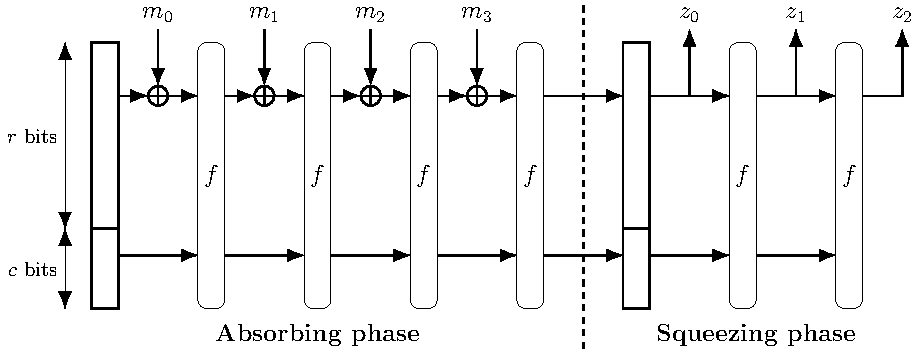
\includegraphics[width=\textwidth]{figures/app_crypto/sponge/sponge.pdf}
\caption[Cryptographic hash function built with Sponge construction]{Here
    is an example of the sponge construction.
    Based on a diagram from~\cite{TikZ:for:Cryptographers}.
    Here, the message $m$ is first padded so that its total length
    is a multiple of the rate $r$.
    The sponge then absorbs the message into its internal state.
    After this, the desired output is squeezed out.}
\label{fig:sponge_construction}
\end{figure}
